\documentclass{cmspaper}
\usepackage{lineno}
\usepackage{amsfonts,amsmath,amssymb}
\usepackage[dvips]{graphicx}
\usepackage{bm}
\usepackage{multirow}
\usepackage{subfigure}  % use for side-by-side figures
%\usepackage[a4paper]{hyperref}

\def\etmiss{\big\slash\hspace{-1.6ex}{E_\text{T}}}
\def\etmissB{\big\slash\hspace{-1.6ex}{\boldsymbol{E}_\text{T}}}
\def\exmiss{\big\slash\hspace{-1.6ex}{E_{x}}}
\def\eymiss{\big\slash\hspace{-1.6ex}{E_{y}}}
\def\sumet{\sum{E_\text{T}}}
\def\sumetB{\sum{\boldsymbol{E}_\text{T}}}

\begin{document}
\begin{linenumbers}


\begin{titlepage}

  % select one of the following and type in the proper number:

%  \cmsnote{2010/001}
  \internalnote{2005/000}
%  \conferencereport{2005/000}
%  \cmsan{2010/029}
%  \cmsdtnote{2005/000}
%  \cmspas{2005/000}
   \date{\today}

  \title{Results of visual scan of high $\etmiss$ events in 7 TeV pp collision data}

  \begin{Authlist}
    A.~Apresyan
    \Instfoot{caltech}{California Institute of Technology, Pasadena, CA, USA}
    D.~Ferencek, F.~Santanastasio %\Aref{a}
   \Instfoot{umd}{University of Maryland, College Park, MD, USA}   
  \end{Authlist}

% if needed, use the following:
%\collaboration{CMS collaboration}

%\Anotfoot{a}{Also at \textit{California Institute of Technology, Pasadena, CA, USA}}

  \begin{abstract}    
   We present the results of a visual scan of high $\etmiss$ events 
   (tc$\etmiss>60$~GeV OR pf$\etmiss>60$~GeV)
   in an inclusive sample of XX~nb$^{-1}$ of 7 TeV pp collision data, 
   after applying the official noise clean-up available in CMSSW\_3\_7\_0\_patch2. 
   The scan is performed separately for events with tc$\etmiss>60$~GeV and pf$\etmiss>60$~GeV
   since the noise clean-up is implemented differently in the two $\etmiss$ algorithms.
   The CMS software {\it Fireworks} has been used to produce the event displays. 
   The high $\etmiss$ events have been visually inspected and classified in different 
   cathegories. The results of this scan can provide hints to further improve the noise 
   cleaning and to identify possible problems and inconsistencies in the algorithms employed 
   in CMS for the $\etmiss$ reconstruction.
  \end{abstract} 

% if needed, use the following:
%\conference{Presented at {\it Physics Rumours}, Coconut Island, April 1, 2005}
%\submitted{Submitted to {\it Physics Rumours}}
%\note{Preliminary version}
  
\end{titlepage}

\setcounter{page}{2}%JPP

\tableofcontents

\clearpage

\section{Introduction}

Commissioning studies performed with test beams, cosmic runs and 
early 0.9~TeV, 2.36~TeV and 7~TeV pp 
collision data have identified several sources of anomalous noise 
(i.e. noise not produce solely from expected fluctuations in the electronics)
in the calorimeters of the CMS experiment:
\begin{itemize}
\item {\it ECAL barrel spikes} - More details are available at XXX.
%Energy deposits in individual channels 
%affected by the noise are cleaned using both topological and 
%timing information of the reconstructed hits. This type of noise is correlated with collisions. 

\item {\it HF PMT hits} - More details are available at~\cite{Chatrchyan:1225105},XXX.
%Energy deposits in individual channels 
%affected by the noise are cleaned using both topological and 
%timing information of the reconstructed hits. PMT hit noise is correlated with collisions. 

\item {\it IonFeedback/HPD/RBX noise in HCAL barrel and endcaps} - More details are available at XXX.
%Events with identified 
%HPD/RBX noise are removed from the analysis using a filter based on both topological 
%and timing information of the reconstructed energy deposits. IonFeedback noise has also been observed 
%but typically affect a few channels and produces low energy signals. A cleaning for IonFeedback noise 
%is not yet available. HPD/RBX noise is not correlated with collisions. 
\end{itemize}
In addition, machine-induced background, in the form of 
beam halo [XXX] and beam scraping events [XXX], have been observed. 

The overlap of either anomalous noise or machine-induced background 
with a pp collision event produces an unbalance in 
the reconstructed missing transverse energy in the event, which can produce 
large tails in the $\etmiss$ distribution. 

We present the results of a visual scan of high $\etmiss$ events 
(tc$\etmiss>60$~GeV OR pf$\etmiss>60$~GeV)
in an inclusive sample of XX~nb$^{-1}$ of 7 TeV pp collision data, 
after applying the official noise clean-up available in CMSSW\_3\_7\_0\_patch2.
The full selection criteria are described in Section~\ref{sec:EventSelection}). 
The scan is performed separately for events with tc$\etmiss>60$~GeV and pf$\etmiss>60$~GeV
since the noise clean-up is implemented differently in the two $\etmiss$ algorithms.
The CMS software {\it Fireworks} [XXX] has been used to produce the event displays. 
The high $\etmiss$ events have been visually inspected and classified in different 
categories. The results of this scan can provide hints to further improve the noise 
cleaning and to identify possible problems and inconsistencies in the algorithms employed 
in CMS for the $\etmiss$ reconstruction.


\section{Datasample, Event Selection, and Noise Cleaning} \label{sec:EventSelection}

{\bf Dataset and CMSSW release:}
\begin{itemize}
\item dataset: /MinimumBias/Commissioning10-GOODCOLL-Jun9thSkim\_v1/RECO
\item CMSSW release: CMSSW\_3\_7\_0\_patch2
\end{itemize}

{\bf Event selection:}
\begin{itemize}
\item Physics declared bit
\item BPTX bit 0
\item Removal of events with large pixel cluster multiplicity
\item Good primary vertex
\item Good Run/LS selection. JSON file: Cert\_132440-136119\_7TeV\_May27thReReco\_Collisions10\_JSON.txt  
\end{itemize}
%More details at [XXX].

{\bf Noise cleaning}

Noise cleaning/event filter for calotower-based $\etmiss$ algorithms (Calo$\etmiss$ and tc$\etmiss$):
\begin{itemize}
\item ECAL barrel spikes (reject RecHits): topology (kWeird flag = swiss cross variable) + timing (kOutOfTime flag)~\cite{ECALAt7TeV};
\item HF PMT hits (reject Rechits): topology (HFLongShort flag = PET+S9/S1) + pulse shape (HFDigiTime flag)~\cite{HFDN};
\item HPD/RBX noise in HBHE (reject events): combination of pulse shape and topological variables~\cite{HCALWGNOTE}.
\end{itemize}

Noise cleaning (reject RecHits) for pf$\etmiss$ is described at~\cite{PFPAS2010}. Timing and topology are used to reject RecHits 
affected by ECAL and HF noise. Topology only is used to reject rechits affected by HBHE noise. No events are rejected.

NOTE: The HPD/RBX noise filter is applied for the scan of both tc$\etmiss$ and pf$\etmiss$ tails presented in this note, 
in order to have the same number of events passing the selection.

Figure~\ref{fig:calomet} shows the cleaned tc$\etmiss$ and pf$\etmiss$ distributions for $\approx 60$~M events 
(precisely 58821832 events) passing the event selection described above.
\begin{figure}[h]
 \centering
 \begin{tabular}{ll}
   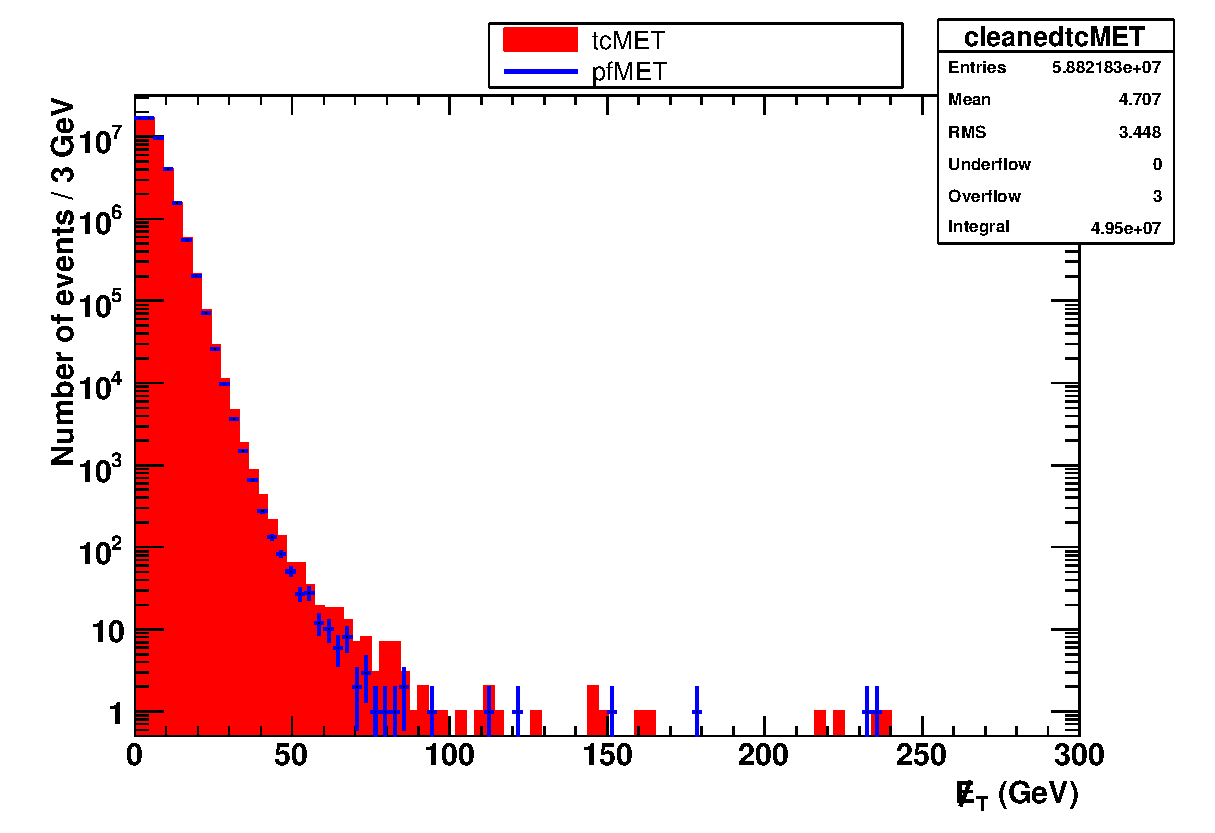
\includegraphics[width=0.7\textwidth]{fig/met.eps} 
 \end{tabular}
\caption{tc$\etmiss$ and pf$\etmiss$ distributions of 7 TeV collision data after applying the full event selection and noise cleaning.}
\label{fig:calomet}
\end{figure}

\section{Scan of high $\etmiss$ events}

The high $\etmiss$ events have been divided in three mutually exclusive categories and stored in the directory \\ 
SKIMDIR = /castor/cern.ch/user/s/santanas/MET/Skims/METtails\_45GeVcut\_May27\_2010/ :
\begin{itemize}
\item Category 1 \quad - \quad Calo$\etmiss>45$~GeV \quad AND \quad tc$\etmiss>45$~GeV\\ 
Root file in RECO format at: \\ SKIMDIR/picked\_events\_CaloMET\_and\_tcMET\_gt\_45GeV\_Artur.root
\item Category 2 \quad - \quad Calo$\etmiss>45$~GeV \quad AND \quad tc$\etmiss<45$~GeV \\
Root file in RECO format at: \\ SKIMDIR/picked\_events\_CaloMET\_gt\_45GeV\_Artur.root
\item Category 3 \quad - \quad Calo$\etmiss<45$~GeV \quad AND \quad tc$\etmiss>45$~GeV \\
Root file in RECO format at: \\ SKIMDIR/picked\_events\_tcMET\_gt\_45GeV\_Artur.root
\end{itemize}

A visual scan of these events have been performed using the CMS event display
software ``Fireworks''. It should pointed out that the results of a visual scan 
are subject to personal judgment. Nevertheless, they should provide
with good approximation a realistic picture of which are the events that populates the tails
of the $\etmiss$ after applying the current noise clean-up.

The result of the scan are summarized in the following sub-sections.

\subsection{Category 1: Calo$\etmiss>45$~GeV AND tc$\etmiss>45$~GeV}

\subsection{Category 2: Calo$\etmiss>45$~GeV AND tc$\etmiss<45$~GeV}

\subsection{Category 3: Calo$\etmiss<45$~GeV AND tc$\etmiss>45$~GeV}
\section{Description and event displays of high $\etmiss$ events} \label{EventDisplay}

\subsection{EB, spike at EB-EE boundary}
We see EB spikes occurring at the boundary between ECAL barrel and endcaps.

The ECAL spikes topological cuts employed in the calotower-based cleaning for tc$\etmiss$ 
are not currently applied to identify ``spikes'' candidates occurring at the boundary between ECAL barrel and endcaps. 
Spikes at the EB-EE boundary could anyway be removed by the timing cuts. Nevertheless, some of them still survives 
after the noise clean-up, as the event shown in Figure~\ref{fig:EBspikeAtBorder}.
It has been verified that all 22 spikes at EB-EE border reported in the tc$\etmiss$ scan are in fact reconstructed in-time, 
and therefore not removed.

All the observed EB spikes at EB-EE boundaries are instead cleaned by PF cleaning. 
The topological cuts applied at the EE/EB boundaries and in
the vicinity of inter-module cracks are tighter than elsewhere, such that they are 
as selective as in the fiducial ECAL region. 

\subsection{EB, EE spikes}
We see one event with an isolated spike in ECAL barrel (EB) far from the EB-EE boundaries 
(Figure~\ref{fig:EBEEspike}, left plot) and two events with an isolated spike in ECAL 
endcap (EE) (one of them in Figure~\ref{fig:EBEEspike}, right plot).

Calotower-based cleaning for spikes is not applied in EE (it is understood that 
spikes are due to particles hitting an APD, which are mounted only in the ECAL barrel). 
The case of EB spike, far from the EB-EE boundary and not cleaned, should be investigated.

All events are cleaned by PF; note that a topological cleaning for spikes is applied by default also in EE.

\subsection{HF, multi-PMT-hits or phi-strip events}
These events are characterized by several anomalous hits in adjacent cells; sometimes they show up as
a strip of hits at the same $i\phi$ location, as the ones reported in Figure~\ref{fig:HFmultiHits}. 
This type of noise cannot be cleaned by the existing topological algorithms in the calotower cleaning 
but could be cleaned by the timing or pulse shape based 
cleaning if hits are out-of-time or have a malformed pulse shape. 
A topological cleaning based on the multiplicity of hits above certain energy threshold 
at the same $i\phi$ location might be effective at identifying such noise.
The source of such events is not yet fully understood.

Some of these events are identified by PF cleaning, but not by calotower cleaning, mainly for two reasons:
\begin{itemize}
\item PF cleaning uses an $E_S$/$E_L$-type variable for long fibers (note: this cut, even being more aggressive on isolated photons 
than the S$9$/S$1$-type variable, it is still safe for physics thanks to the presence of an {\it a posteriori} recovery algorithm
implemented in the PF cleaning);
\item in the PF cleaning, the timing is first applied, and the topological cleaning is applied once 
the timing-cleaned hits are removed, making it effective on multi hits. 
Work is ongoing to implement such cleaning procedure in CMSSW\_3\_8\_X for the calotower cleaning as well.
\end{itemize}
%Studies are ongoing to understand the differences.

\subsection{HF, double-PMT-hits}
These events are characterized by significant energy in both long and short fibers in a single
isolated tower, as shown in Figure~\ref{fig:HFdoublehits}. For high $\etmiss$ events, 
this noise often shows up in the towers located at the smallest $\eta$ 
value in HF ($\eta$=3). This can be explained by the fact that, for a given energy, 
a noise occurring at smaller $\eta$ produces a larger transverse energy, and therefore is more visible at high $\etmiss$.
Anyway it's not excluded that double-hits occurs also at larger $\eta$; but in this case such events might 
fall in the bulk of $\etmiss$ distribution.

This type of noise cannot be cleaned by the current topological algorithms (PET or S9/S1) used in calotower cleaning 
but can be cleaned by the timing or pulse shape based cleaning if hits are out-of-time or have a malformed pulse shape.
However, cases of in-time double-hits with good pulse shape have been observed. In such cases, a cleaning based on
S$8$/S$1$ isolation variable could be effective, where S$8$/S$1$ is defined in a similar way to S$9$/S$1$
with the companion RecHit energy from the same HF tower left out from the sum. 
%On the other hand, this type of cleaning is not expected to be fully safe for isolated particles, 
%in particular for physically bigger towers at lower $\eta$ values. 
%Preliminary studies on the use of S$8$/S$1$ isolation variable have been performed. 

PF cleaning flags most of these noise events. 
The HF double-hits removed by PF cleaning are characterized by having 
energy in the short fiber larger than the energy in the long fiber. 
If, in addition to this condition, the HF tower is also isolated 
(i.e. small energy in the adjacent towers), the double-hit is identified by the PF cleaning algorithm.
No such algorithm is implemented for calotower cleaning in the release CMSSW\_3\_7\_0\_patch2; 
work is ongoing to include it in CMSSW\_3\_8\_X.
%Studies are ongoing to understand the differences
%with calotower-based cleaning.

\subsection{HF, PMT hit embedded in a jet} ~\label{sec:HFHitEmbeddedInJet}
These events are characterized by one or more anomalous hits embedded inside a jet (or simply not isolated), 
as shown in Figure~\ref{fig:HFhitEmbeddedInJet}. This type of noise could arise from muons coming from 
in-flight decays of hadronic particles or from a jet punch-through. In both cases
such jets could be identified using the JetID variables since it is expected that a large fraction of the
total jet energy would come from only one or two HF towers. Due to an overlap between real and anomalous signal there are
two cleaning strategies possible: an entire event could be rejected or a more sophisticated anomalous energy
subtraction algorithm would have to be developed.

Neither calotower-based cleaning nor PF cleaning are able to identify these noise events 
(with the exception of one event removed by PF cleaning and not by calotower cleaning).

\subsection{HBHE, IonFeedback/HPD/RBX noise}
These events are characterized by low multiplicity noise or single noisy channels in HCAL barrel or endcap.
Two examples are shown in Figure~\ref{fig:HBHEnoise}.
Improved timing cuts could be employed to identify these residual noise events.

Neither calotower-based cleaning nor PF cleaning are able to identify these residual HBHE noise events.

\subsection{Physics}
It is observed that approximately 30\% of the high $\etmiss$ events don't contain an obvious source of noise
(and therefore are classified as ``Physics''). They are typically multi-jet events where 
the large fake $\etmiss$ is produced by jet energy mis-measurements or jets at the boundaries between sub-detectors, 
but can also be events with real $\etmiss$. Figure~\ref{fig:Physics} 
shows some examples of physics events with large $\etmiss$. 

In about 50\% of high tc$\etmiss$ events with multi-jet topology, pf$\etmiss$ values are 
smaller than tc$\etmiss$ values. More details can be found in 
the Tables~\ref{tab:tcMETskim} and ~\ref{tab:pfMETskim}, and in the list of events posted at the end of the note.
The events are classified based on the jet multiplicity using caloJets with uncorrected $p_T>10$~GeV.

\subsection{Others, large muon-induced pf$\etmiss$}
We observed 5 events with large pf$\etmiss$ (sometimes a few hundreds GeV) 
but very small tc$\etmiss$. 
The muon is reconstructed as ``global muon'' and ``standalone muon'', 
but not as ``tracker muon''. An example is shown in Figure~\ref{fig:largeMuonInducedPfMET}.

Four of these events have pf$\etmiss>80$~GeV, with pf$\etmiss$ = 83, 242, 337
and 528 GeV, respectively, and a muon with $|\eta| > 2.2$. 
These muons have all an inner tracker track associated to them. 
They are indeed not ``tracker muon'', meaning that they fail the tracker-muon
criteria, but they are all global muons (with a track and a stand-alone
muon part) for which the reco::muon pt is not correct. The track is found to be
not well reconstructed (which points to tracker alignment problem or geometry in this large eta region).
Using the global muon momentum instead of the track momentum in the pf$\etmiss$ reconstruction
cleans these four events. This change will be implemented in PF for CMSSW\_3\_8\_X, 
while waiting for an improvement of the tracking/alignment.

%What is interesting is that such poorly reconstructed muons are not seen
%in the simulation, which points to something odd in the muon and or
%tracker alignment or geometry in this large eta region.

%
\begin{figure}[h]
 \centering
% \begin{tabular}{ll}
   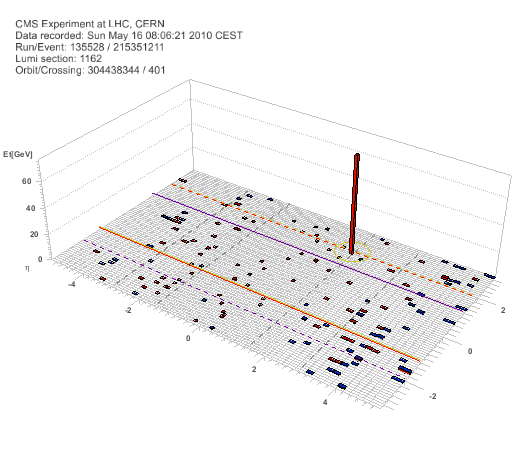
\includegraphics[width=0.47\textwidth]{fig/EBspikeAtBorder.png} 
% \end{tabular}
\caption{Example of an ``EB spike at EB-EE boundary'' event}
\label{fig:EBspikeAtBorder}
\end{figure}

%
\begin{figure}[h]
 \centering
 \begin{tabular}{ll}
   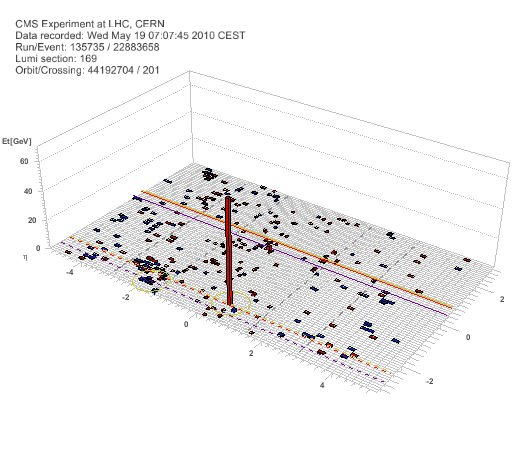
\includegraphics[width=0.47\textwidth]{fig/EBspike.png} &
   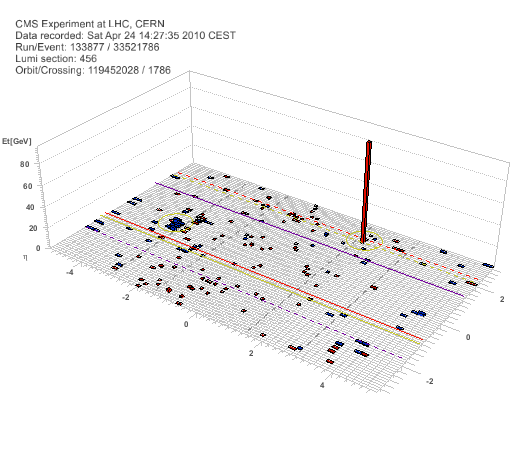
\includegraphics[width=0.47\textwidth]{fig/EEspike.png} \\
 \end{tabular}
\caption{Example of an ``EB spike'' (left) and an ``EE spike'' (right) event}
\label{fig:EBEEspike}
\end{figure}


%
\begin{figure}[h]
 \centering
 \begin{tabular}{ll}
   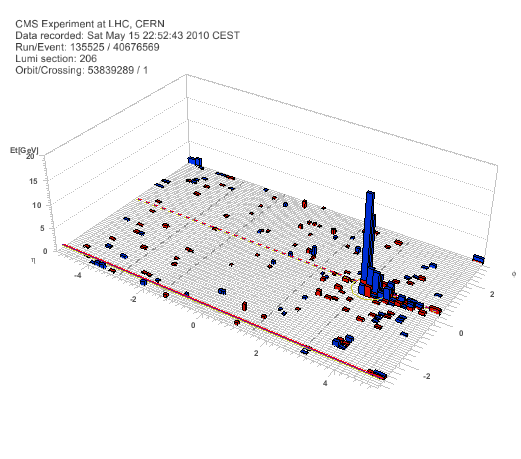
\includegraphics[width=0.47\textwidth]{fig/HFmultiHits.png} &
   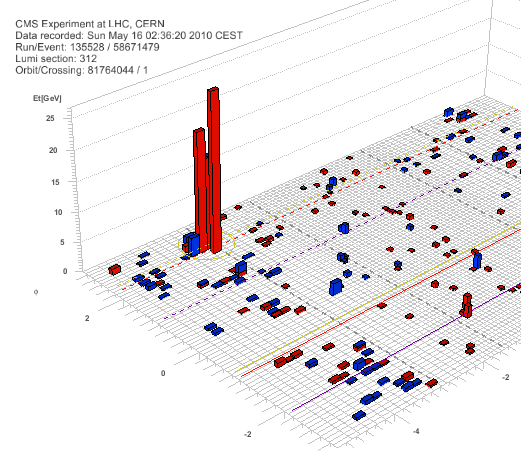
\includegraphics[width=0.47\textwidth]{fig/HFmultiHits_2.png} \\
 \end{tabular}
\caption{Example of two ``HF multi-PMT-hits or phi-strip'' events}
\label{fig:HFmultiHits}
\end{figure}

%
\begin{figure}[h]
 \centering
 \begin{tabular}{ll}
   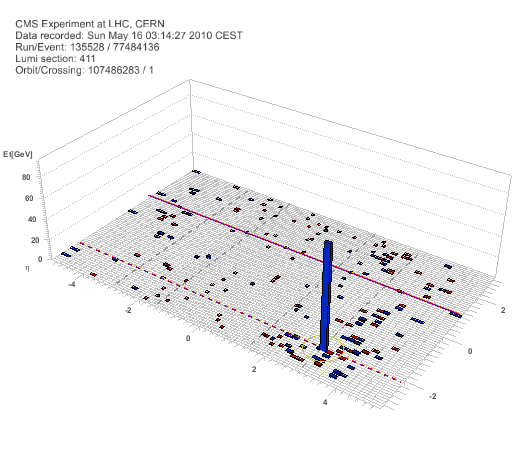
\includegraphics[width=0.47\textwidth]{fig/HFdoubleHit.png} &
   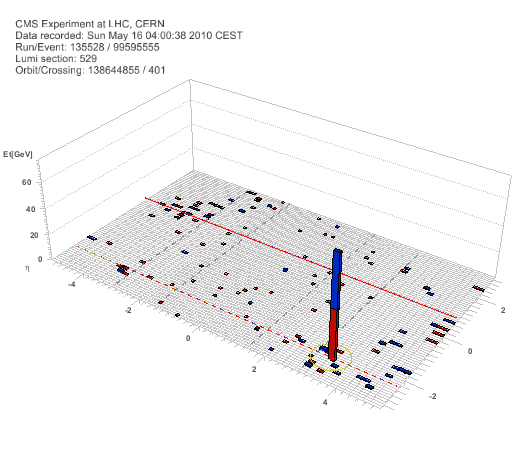
\includegraphics[width=0.47\textwidth]{fig/HFdoubleHit_1.png} \\
 \end{tabular}
\caption{Example of two ``HF double-PMT-hits'' events. Event in left plot is cleaned by PF and not by 
calotower-based cleaning; the event on the right is not cleaned by any of the two. 
NOTE: The event display for the left plot is mis-leading since the hit is not single, 
as it seems, but double. In fact, in this event display (produce with Fireworks) 
the following convention is used for HF towers: blue=2*$E_{S}$=hadEnergy, while red=$E_{L}-E_{S}$=emEnergy. 
In this event the emEnergy (``red'') is negative, but both energies in long and short fibers, $E_{L}$ and $E_{S}$, are large
(several hundreds of GeV). The event display only shows positive quantities 
(only the hadEnergy = ``blue''), so the ``negative'' red spike is not visible and it gives the illusion of a single hit. 
It is observed that most of double-hits cleaned by PF cleaning have negative emEnergy, i.e. $E_S>E_L$.}
\label{fig:HFdoublehits}
\end{figure}

%
\begin{figure}[h]
 \centering
 \begin{tabular}{ll}
   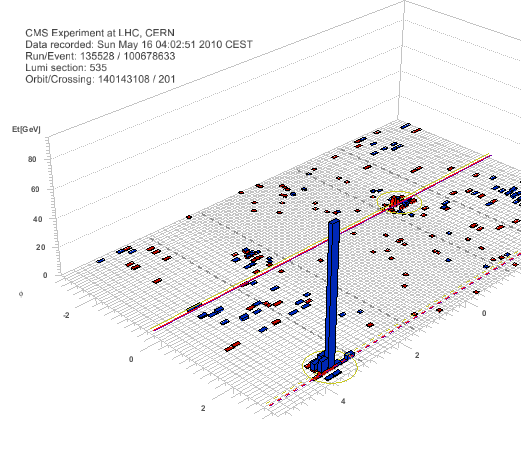
\includegraphics[width=0.47\textwidth]{fig//HFhitInJet.png} & 
   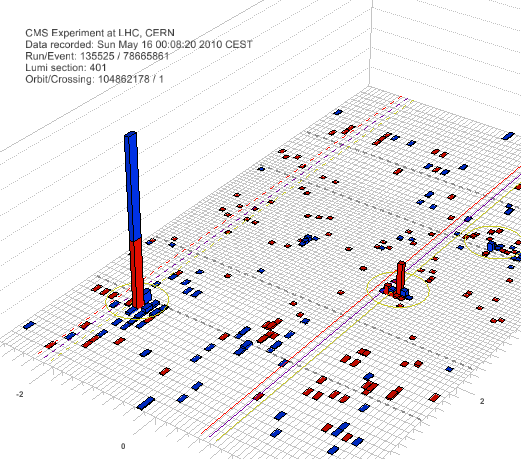
\includegraphics[width=0.47\textwidth]{fig//HFhitInJet_1.png} \\
 \end{tabular}
\caption{Example of two ``HF PMT hit embedded in a jet'' events}
\label{fig:HFhitEmbeddedInJet}
\end{figure}

%
\begin{figure}[h]
 \centering
 \begin{tabular}{ll}
   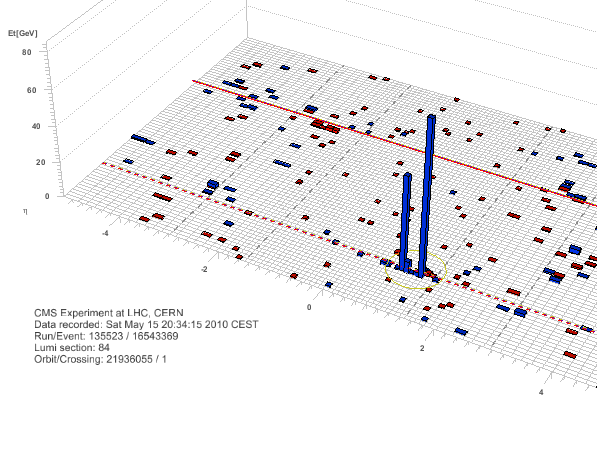
\includegraphics[width=0.47\textwidth]{fig/HBHEnoise_lowMult.png} &
   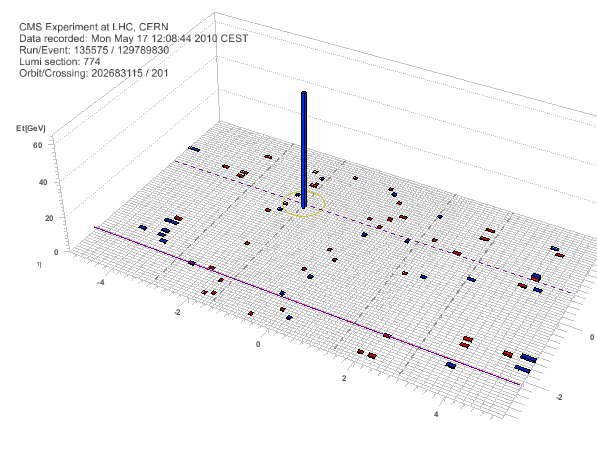
\includegraphics[width=0.47\textwidth]{fig/HBHEnoise_spike.png} \\
 \end{tabular}
\caption{Example of two ``HBHE IonFeedback/HPD/RBX'' noise events. 
The left plot shows an HPD/RBX noise event with low hit multiplicity. 
The right plot show instead an isolated spike, 
probably IonFeedback noise affecting an individual channel.}
\label{fig:HBHEnoise}
\end{figure}

%
\begin{figure}[h]
 \centering
 \begin{tabular}{ll}
   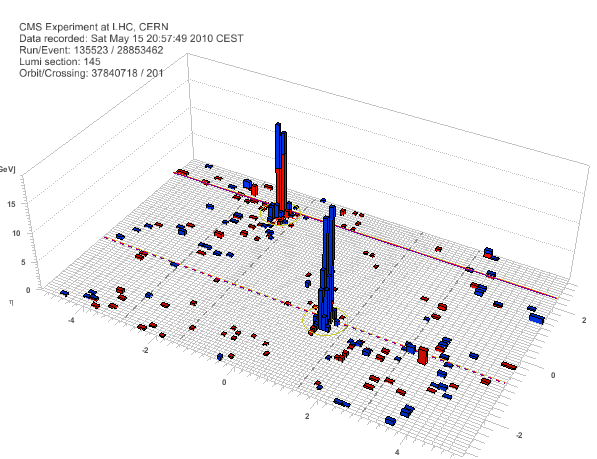
\includegraphics[width=0.47\textwidth]{fig/Physics2.png} &
   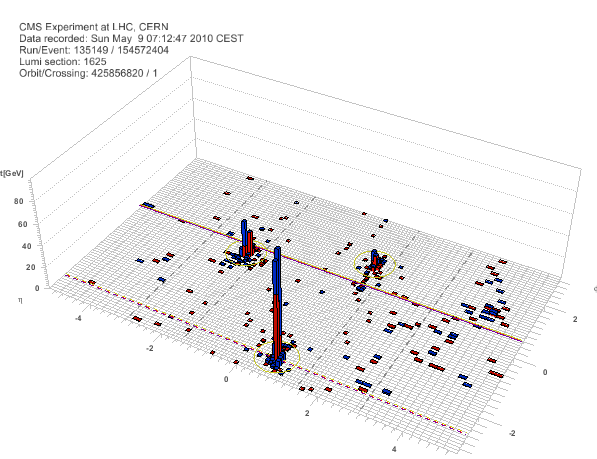
\includegraphics[width=0.47\textwidth]{fig/Physics3.png} \\
   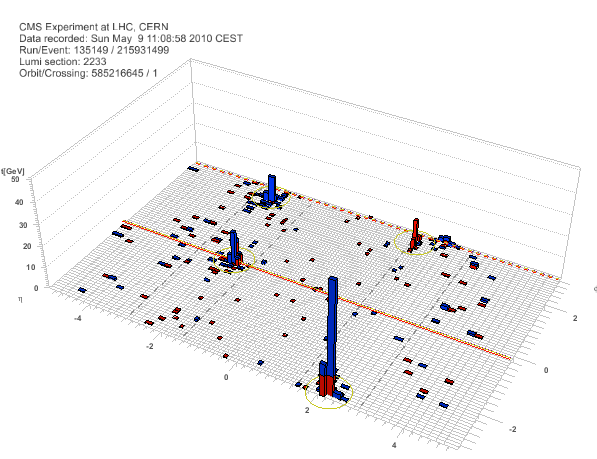
\includegraphics[width=0.47\textwidth]{fig/Physics4.png} &
   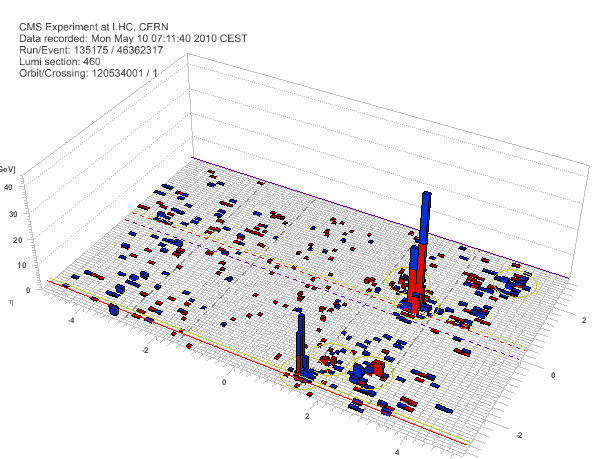
\includegraphics[width=0.47\textwidth]{fig/Physics6.png} \\
 \end{tabular}
\caption{Example of ``Physics'' events with multi-jet topology}
\label{fig:Physics}
\end{figure}

%
\begin{figure}[h]
 \centering
 \begin{tabular}{ll}
   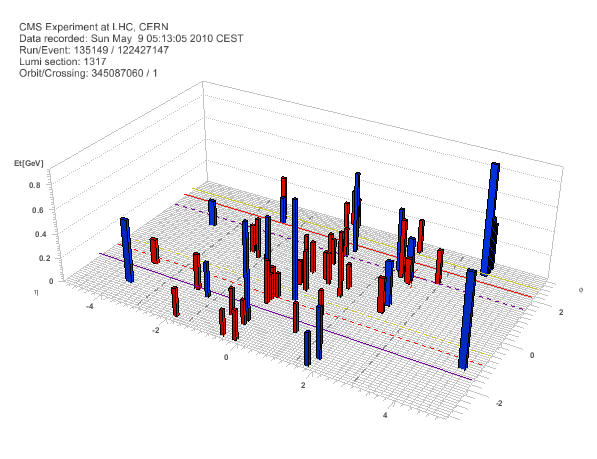
\includegraphics[width=0.47\textwidth]{fig/largeMuonInducedPfMET.png} &
   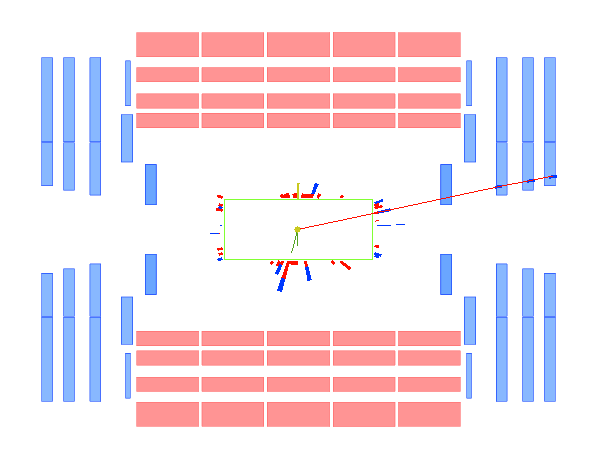
\includegraphics[width=0.47\textwidth]{fig/largeMuonInducedPfMET_1.png} \\
 \end{tabular}
\caption{Example of a ``large muon-induced pf$\etmiss$'' event
shown in the eta/phi view (left) and in the transverse plane view (right). There is an high $p_{T}$ 
muon reconstructed as ``global muon'' and ``standalone muon'' , but not as ``tracker muon''.}
\label{fig:largeMuonInducedPfMET}
\end{figure}





\clearpage
\section{List of high $\etmiss$ events}

In this section, the complete list of high $\etmiss$ events is provided, for both tc$\etmiss$ 
(Table~\ref{tab:tcMETlist1}, ~\ref{tab:tcMETlist2}, ~\ref{tab:tcMETlist3} ) and pf$\etmiss$ 
(Table~\ref{tab:pfMETlist1}) skims.


% tcMET list Part 1
\begin{table}[htbp]
  \begin{center}
    \begin{tabular}{|c|c|c|c|c|}
      \hline
      Run & Event & LS & tc$\etmiss$ & category \\     
      \hline
      132599 & 4345895     & 183  &    78.2843  & HF multi-PMT-hits or phi-strip events (large pfMET) \\
      132601 & 166842      & 7    &    81.8343  & HF double-PMT-hits  (small pfMET) \\
      132601 & 4585263     & 188  &    237.387  & EB spike at EB-EE boundary (small pfMET) \\
      132658 & 892391      & 37   &    68.8251  & Physics 2 jets (small pfMET) \\
      133046 & 3187891     & 138  &    148.51   & EB spike at EB-EE boundary (small pfMET) \\
      133321 & 14516033    & 238  &    60.4839  & HF double-PMT-hits  (small pfMET) \\
      133874 & 41569953    & 528  &    81.4559  & HE noise (large pfMET) \\
      133874 & 66583217    & 826  &    85.6937  & HF double-PMT-hits  (large pfMET) \\
      133877 & 21558793    & 299  &    83.5564  & HF double-PMT-hits  (small pfMET) \\
      133877 & 33521786    & 456  &    90.3345  & EE spike (small pfMET) \\
      133877 & 83377798    & 1130 &    63.9341  & HF double-PMT-hits  (large pfMET) \\
      133885 & 335989      & 5    &    62.133   & Physics 3 jets (large pfMET) \\
      133927 & 369683      & 6    &    93.0333  & HF double-PMT-hits  (small pfMET) \\
      133928 & 22682366    & 319  &    63.7869  & HF multi-PMT-hits or phi-strip events (large pfMET) \\
      133928 & 36620099    & 517  &    66.8677  & Physics 1 jet (large pfMET) \\
      135149 & 63603939    & 753  &    66.9592  & Physics 2 jets (small pfMET) \\
      135149 & 116927949   & 1265 &    63.1608  & Physics 3 jets (large pfMET) \\
      135149 & 154572404   & 1625 &    98.3469  & Physics 3 jets (large pfMET) \\
      135149 & 155186256   & 1631 &    60.8672  & Physics 3 jets (large pfMET) \\
      135149 & 156347129   & 1642 &    65.4799  & HF double-PMT-hits (small pfMET) \\
      135149 & 162208514   & 1699 &    78.278   & HF multi-PMT-hits or phi-strip events (large pfMET) \\ 
      135149 & 214116071   & 2215 &    66.5431  & HF PMT hit embedded in a jet (large pfMET) \\
      135149 & 215931499   & 2233 &    71.0733  & Physics 4 jets (large pfMET) \\
      135149 & 217153658   & 2245 &    81.4574  & Physics 3 jets (large pfMET) \\
      135149 & 222730662   & 2307 &    418.801  & EB spike at EB-EE boundary (small pfMET) \\ 
      135149 & 233103931   & 2411 &    74.2742  & EB spike at EB-EE boundary (small pfMET) \\ 
      135149 & 267019811   & 2758 &    66.3561  & Physics 4 jets (small pfMET) \\
      135149 & 318396401   & 3297 &    542.981  & EB spike at EB-EE boundary (small pfMET) \\
      135175  & 17812005     & 191  &    64.2943 & HB noise (large pfMET) \\
      135175  & 42757899     & 426  &    92.0741 & HF double-PMT-hits (small pfMET) \\
      135175  & 46362317     & 460  &    69.9842 & Physics 6 jets (tcMET ~ 2 * pfMET) \\
      135175  & 57982991     & 574  &    73.1318 & HF double-PMT-hits (small pfMET) \\
      \hline
    \end{tabular}
    \caption{List of events with tc$\etmiss>60$~GeV - Part 1.}        
    \label{tab:tcMETlist1}
  \end{center}
\end{table}


% tcMET list Part 2
\begin{table}[htbp]
  \begin{center}
    \begin{tabular}{|c|c|c|c|c|}
      \hline
      Run & Event & LS & tc$\etmiss$ & category \\     
      \hline
      135175  & 64940222     & 641  &    62.4991 & EB spike at EB-EE boundary (small pfMET) \\
      135175  & 72861680     & 718  &    116.591 & EB spike at EB-EE boundary (small pfMET) \\
      135175  & 94014613     & 926  &    145.352 & Physics 4 jets (tcMET ~ 2 * pfMET) \\
      135175  & 100575970    & 990  &    61.3085 & HF double-PMT-hits (large pfMET) \\
      135521  & 22453149     & 203  &    71.9826 & Physics 3 jets (large pfMET) \\
      135521  & 32219215     & 251  &    69.445  & Physics 2 jets (large pfMET) \\
      135521  & 40089571     & 289  &    77.7739 & EB spike at EB-EE boundary (small pfMET) \\
      135521  & 66824775     & 420  &    80.9651 & EB spike at EB-EE boundary (small pfMET) \\
      135521  & 69919879     & 435  &    80.0659 & HF multi-PMT-hits or phi-strip events (small pfMET), eta strip \\
      135523  & 9879701      & 50   &    61.4423 & HF double-PMT-hits (small pfMET) \\
      135523  & 16543369     & 84   &    164.131 & HB noise (large pfMET) \\
      135523  & 28853462     & 145  &    64.5248 & Physics 2 jets (large pfMET) \\
      135525  & 17433547     & 87   &    68.2453 & Physics 3 jets (small pfMET), pfMET = 7 GeV \\ 
      135525  & 40676569     & 206  &    62.4033 & HF multi-PMT-hits or phi-strip events (large pfMET), 2-4 phi strip \\
      135525  & 45035068     & 228  &    70.4362 & EB spike at EB-EE boundary (small pfMET) \\
      135525  & 48804509     & 247  &    62.6639 & Physics 4 jets (large pfMET) \\
      135525  & 63386076     & 320  &    77.1017 & HF multi-PMT-hits or phi-strip events (large pfMET) \\
      135525  & 78665861     & 401  &    62.0925 & HF PMT hit embedded in a jet (large pfMET) \\
      135525  & 80550953     & 410  &    65.2472 & Physics 2 jets (tcMET ~ 2 * pfMET) \\
      135525  & 87558102     & 448  &    110.215 & Physics 5 jets (large pfMET) \\ 
      135525  & 88031668     & 450  &    64.1569 & Physics 4 jets (small pfMET) \\
      135528  & 884119       & 5    &    62.3458 & HF double-PMT-hits (large pfMET) \\
      135528  & 19813983     & 105  &    61.8938 & HF multi-PMT-hits or phi-strip events (large pfMET) \\
      135528  & 32603499     & 174  &    63.8757 & EB spike at EB-EE boundary (small pfMET) \\
      135528  & 58671479     & 312  &    64.5086 & HF multi-PMT-hits or phi-strip events (small pfMET) \\
      135528  & 60003196     & 319  &    74.3878 & Physics 2 jets (small pfMET) \\
      135528  & 77484136     & 411  &    89.8829 & HF double-PMT-hits (small pfMET) \\
      135528  & 80490418     & 426  &    73.026  & Physics 3 jets (tcMET ~ 2 * pfMET) \\
      135528  & 99595555     & 529  &    82.2867 & HF double-PMT-hits (large pfMET) \\
      135528  & 100678633    & 535  &    78.523  & HF PMT hit embedded in a jet (large pfMET) \\
      135528  & 102808626    & 546  &    68.4343 & Physics 6 jets (tcMET ~ 2 * pfMET) \\
      135528  & 115447830    & 618  &    62.2738 & HB noise (large pfMET) \\
      135528  & 130731462    & 699  &    127.18  & HF double-PMT-hits (small pfMET) \\
      \hline
    \end{tabular}
    \caption{List of events with tc$\etmiss>60$~GeV - Part 2.}        
    \label{tab:tcMETlist2}
  \end{center}
\end{table}


% tcMET list Part 3
\begin{table}[htbp]
  \begin{center}
    \begin{tabular}{|c|c|c|c|c|}
      \hline
      Run & Event & LS & tc$\etmiss$ & category \\     
      \hline
      135528  & 150342996    & 808  &    66.7701 & Physics 5 jets (tcMET ~ 2 * pfMET) \\
      135528  & 153336127    & 824  &    63.8531 & Physics 4 jets (large pfMET) \\
      135528  & 162079374    & 871  &    111.931 & HF multi-PMT-hits or phi-strip events (small pfMET) \\
      135528  & 172155075    & 927  &    216.754 & EB spike at EB-EE boundary (small pfMET) \\
      135528  & 178385490    & 960  &    113.215 & HF multi-PMT-hits or phi-strip events (small pfMET) \\
      135528  & 194937806    & 1049 &    61.32   & Physics 4 jets (large pfMET) \\
      135528  & 195017684    & 1050 &    65.1985 & HF double-PMT-hits (small pfMET) \\
      135528  & 204463628    & 1103 &    69.0627 & Physics 2 jets (small pfMET) \\
      135528  & 207348623    & 1118 &    75.5706 & HF multi-PMT-hits or phi-strip events (large pfMET) \\ 
      135528  & 215351211    & 1162 &    68.9099 & EB spike at EB-EE boundary (small pfMET) \\
      135528  & 226804792    & 1227 &    575.609 & EB spike at EB-EE boundary (small pfMET) \\
      135528  & 227722743    & 1232 &    159.545 & EB spike at EB-EE boundary (small pfMET) \\
      135528  & 238836923    & 1292 &    69.2778 & EB spike at EB-EE boundary (small pfMET) \\
      135528  & 256160509    & 1388 &    74.4981 & EB spike at EB-EE boundary (small pfMET) \\
      135535  & 15564358     & 92   &    224.509 & HB noise (large pfMET) \\
      135535  & 18401448     & 109  &    79.3533 & HF double-PMT-hits (small pfMET) \\
      135535  & 31027189     & 182  &    67.2768 & Others - HB activity + muon (large pfMET) \\
      135573  & 13003948     & 151  &    81.3199 & HF double-PMT-hits (small pfMET) \\
      135575  & 5342229      & 38   &    63.8363 & Physics 3 jets (tcMET ~ 2 * pfMET) \\
      135575  & 11156890     & 79   &    61.2564 & Physics 3 jets (large pfMET) \\
      135575  & 13695733     & 97   &    235.509 & EB spike at EB-EE boundary (small pfMET) \\
      135575  & 64338278     & 393  &    68.2189 & Physics 2 jets (large pfMET) \\
      135575  & 67135767     & 408  &    68.972  & HF multi-PMT-hits or phi-strip events (small pfMET) \\
      135575  & 67221216     & 409  &    78.3203 & EB spike at EB-EE boundary (small pfMET) \\
      135575  & 69788619     & 423  &    63.2861 & Physics 4 jets (large pfMET) \\
      135575  & 93340831     & 559  &    146.205 & Physics 2 jets + muon in jet + EB activity at border? (large pfMET) \\
      135575  & 96504815     & 577  &    60.6013 & EB spike at EB-EE boundary (small pfMET) \\
      135575  & 117083855    & 698  &    86.9326 & HF double-PMT-hits (small pfMET) \\
      135575  & 126932629    & 757  &    72.2135 & HF double-PMT-hits (small pfMET) \\
      135575  & 128277130    & 765  &    64.6596 & Physics 3 jets (tcMET ~ 2 * pfMET) \\
      135575  & 129789830    & 774  &    66.7404 & HB noise (large pfMET), Ion Feedback? \\
      135575  & 130735782    & 779  &    64.1565 & EB spike at EB-EE boundary (small pfMET) \\
      135575  & 134419161    & 805  &    61.4918 & HF double-PMT-hits (small pfMET) \\
      135575  & 144805158    & 870  &    86.8711 & HF double-PMT-hits (small pfMET) \\
      135575  & 149874280    & 901  &    61.6245 & EB spike at EB-EE boundary (small pfMET) \\
      135575  & 180503581    & 1110 &    64.2686 & HF double-PMT-hits (small pfMET) \\
      135575  & 189427985    & 1175 &    61.6306 & Physics 2 jets (tcMET ~ 2 * pfMET) \\
      135575  & 190898956    & 1186 &    73.6522 & EB spike at EB-EE boundary (small pfMET) \\
      135575  & 192395010    & 1197 &    64.455  & Physics 3 jets (tcMET ~ 2 * pfMET) \\
      135575  & 193746493    & 1207 &    104.321 & HB noise (large pfMET) \\
      135735  & 8376298      & 103  &    72.7973 & Physics 4 jets (small pfMET) \\
      135735  & 22883658     & 169  &    83.7303 & EB spike (small pfMET) \\       
      \hline
    \end{tabular}
    \caption{List of events with tc$\etmiss>60$~GeV - Part 3.}        
    \label{tab:tcMETlist3}
  \end{center}
\end{table}



% pfMET list Part 1
\begin{table}[htbp]
  \begin{center}
    \begin{tabular}{|c|c|c|c|c|}
      \hline
      Run & Event & LS & pf$\etmiss$ & category \\     
      \hline
      132599 & 4345895     &  183  &    67.483   & HF multi-PMT-hits or phi-strip events (large tcMET) \\ 
      133874 & 41569953    &  528  &    85.4173  & HE noise (large tcMET) \\
      133874 & 66583217    &  826  &    94.6307  & HF double-PMT-hits  (large tcMET) \\
      133877 & 9967629     &  147  &    63.2921  & Physics 2 jets (large tcMET) \\
      133877 & 83377798    &  1130 &    62.5759  & HF double-PMT-hits  (large tcMET) \\
      133885 & 335989      &  5    &    65.6229  & Physics 3 jets (large tcMET) \\
      133928 & 36620099    &  517  &    67.8891  & Physics 1 jet (large tcMET) \\
      135149 & 116927949   &  1265 &    72.6891  & Physics 3 jets (large tcMET) \\
      135149 & 122427147   &  1317 &    528.658  & Others large muon-induced pfMET, very small caloMET/tcMET \\
      135149 & 154572404   &  1625 &    63.0696  & Physics 3 jets (large tcMET) \\
      135149 & 162208514   &  1699 &    70.1507  & HF multi-PMT-hits or phi-strip events (large tcMET) \\
      135149 & 215931499   &  2233 &    86.0465  & Physics 4 jets (large tcMET) \\
      135149 & 217153658   &  2245 &    67.7884  & Physics 3 jets (large tcMET) \\
      135175 & 57397642    &  568  &    337.561  & Others large muon-induced pfMET, very small caloMET/tcMET \\
      135175 & 94014613    &  926  &    61.3586  & Physics 4 jets (tcMET ~ 2 * pfMET) \\
      135175 & 100575970   &  990  &    61.8675  & HF double-PMT-hits (large tcMET) \\
      135521 & 22774568    &  205  &    60.8714  & Physics 3 jets (large tcMET) \\
      135521 & 32219215    &  251  &    62.8553  & Physics 2 jets (large tcMET) \\
      135523 & 16543369    &  84   &    179.233  & HB noise (large tcMET) \\
      135525 & 48804509    &  247  &    60.366   & Physics 4 jets (large tcMET) \\
      135525 & 63386076    &  320  &    67.772   & HF multi-PMT-hits or phi-strip events (large tcMET) \\
      135525 & 78665861    &  401  &    62.6467  & HF PMT hit embedded in a jet (large tcMET) \\
      135525 & 87558102    &  448  &    121.168  & Physics 5 jets (large tcMET) \\
      135528 & 32056404    &  171  &    231.068  & Others large muon-induced pfMET, very small caloMET/tcMET \\
      135528 & 99411269    &  528  &    62.2593  & HB noise (large tcMET) , Ion Feedback? \\
      135528 & 99595555    &  529  &    80.0732  & HF double-PMT-hits (large tcMET) \\
      135528 & 99860976    &  531  &    69.2713  & Physics 6 jets (pfMET ~ 2*tcMET) \\
      135528 & 100678633   &  535  &    67.2221  & HF PMT hit embedded in a jet (large tcMET) \\
      135528 & 109847963   &  584  &    83.8501  & Others large muon-induced pfMET, very small caloMET/tcMET \\
      135528 & 115447830   &  618  &    72.7202  & HB noise (large tcMET) \\
      135528 & 190129212   &  1023 &    64.6779  & Physics 2 jets + muon (large tcMET) \\
      135528 & 192636869   &  1037 &    66.284   & HF PMT hit embedded in a jet (pfMET ~ 2 * tcMET) \\
      135528 & 207348623   &  1118 &    68.2922  & HF multi-PMT-hits or phi-strip events (large tcMET) \\
      135528 & 208274999   &  1123 &    60.6407  & Others large muon-induced pfMET, very small caloMET/tcMET \\
      135535 & 15564358    &  92   &    235.597  & HB noise (large tcMET) \\
      135535 & 31027189    &  182  &    72.7387  & Others - HB activity + muon (large tcMET) \\
      135575 & 11156890    &  79   &    66.5948  & Physics 3 jets (large tcMET) \\
      135575 & 64338278    &  393  &    64.4694  & Physics 2 jets (large tcMET) \\ 
      135575 & 75318623    &  455  &    60.9222  & Physics jet + muon (large tcMET) \\
      135575 & 93340831    &  559  &    152.727  & Physics 2 jets + muon in jet + EB activity at border? (large tcMET) \\
      135575 & 129789830   &  774  &    76.5243  & HB noise (large tcMET) , Ion Feedback? \\
      135575 & 136780600   &  820  &    64.009   & HB noise (large tcMET) , Ion Feedback? \\
      135575 & 193746493   &  1207 &    112.707  & HB noise (large tcMET) \\
      \hline
    \end{tabular}
    \caption{List of events with pf$\etmiss>60$~GeV.}        
    \label{tab:pfMETlist1}
  \end{center}
\end{table}

%\input{Conclusion}


\end{linenumbers}
\end{document}

